\documentclass[12pt]{article}
\usepackage{latexblog}

% ============================================================
% Blog Metadata
% ============================================================
\blogtitle{Hadoop(2)：单机Hadoop环境安装}
\blogdate{2021-09-29}
\blogtags{Hadoop, 大数据}
\bloglang{zh}
\blogsummary{}

\begin{document}
\makeblogtitle

作为一个从来没接触过大数据的小白，从0开始来学习一下Hadoop。首先是安装环境，官网给出了几种方式:

\begin{itemize}
\tightlist
\item
  Local (Standalone) Mode: 单机版的模式，运行在一个JVM进程
\item
  Pseudo-Distributed Mode: 伪分布式模式，运行多个JVM进程来模拟分布式的环境
\item
  Fully-Distributed Mode: 完全分布式部署在多台机器上
\end{itemize}

当然最理想的当然是真实的分布式部署了，在进行分布式部署之前，先来简单的单机版本部署一下，以便熟悉一下Hadoop相关的概念。

\section{准备}\label{ux51c6ux5907}

\subsection{环境安装}\label{ux73afux5883ux5b89ux88c5}

\subsubsection{VirtualBox}\label{virtualbox}

因为我们的目标是在本机实现分布式的部署，来模拟真实的集群环境，所以需要利用虚拟机来构建多个独立的系统。要做到这步有很多种方式，比如：

\begin{itemize}
\tightlist
\item
  KVM
\item
  VirtualBox
\item
  Multipass
\end{itemize}

其实我最开始尝试过Multipass，这货是Ubuntu推出的感觉比较新的样子，但是我用了一段时间之后莫名的出现了虚拟机无法启动的情况，可能跟MacOS兼容性还不是很好吧。所以比较靠谱和简单的选择是VirtualBox，不仅比较稳定（虽然在Mac上也遇到些Bug），而且还跨平台。

安装VirtualBox非常简单：

\begin{itemize}
\tightlist
\item
  ArchLinux: \texttt{sudo\ pacman\ -S\ virtualbox}
\item
  Mac/Windows: 下直接下载二进制程序安装即可
\end{itemize}

\subsubsection{Vagrant}\label{vagrant}

Virtualbox跟Docker这种容器平台相比一个劣势是系统的安装必须要从头开始。当然自己可以安装完成之后创建一个模板来复制虚拟机，终究比较麻烦。幸好有Vagrant这个工具可以帮助来管理虚拟机，可以快速的从仓库拉取镜像来创建一个虚拟机，以及自动化的配置多个机器、网络、安装脚本等，十分方便。

安装Vagrant:

\begin{itemize}
\tightlist
\item
  ArchLinux: \texttt{sudo\ pacman\ -S\ vagrant}
\item
  Mac: `brew install vagrant
\item
  Windows: 下直接下载二进制程序安装即可
\end{itemize}

安装完成之后，就可以用其来创建虚拟机了。它支持的所有镜像（它的术语叫box）可以在\href{https://app.vagrantup.com}{公开仓库}中找到，后续我们将选用\href{https://app.vagrantup.com/ubuntu/boxes/focal64}{Ubuntu 20.04 LTS官方版本}作为服务器基础镜像。

\subsubsection{下载Hadoop}\label{ux4e0bux8f7dhadoop}

可以从\href{https://mirrors.tuna.tsinghua.edu.cn/apache/hadoop}{清华大学Hadoop镜像}下载Hadoop,当前最新的是\href{https://mirrors.tuna.tsinghua.edu.cn/apache/hadoop/common/hadoop-3.3.1/hadoop-3.3.1.tar.gz}{hadoop-3.3.1}。

\subsection{系统安装}\label{ux7cfbux7edfux5b89ux88c5}

\subsubsection{创建Ubuntu Server}\label{ux521bux5efaubuntu-server}

利用Vagrant命令快速生成一个虚拟机：

\begin{Shaded}
\begin{Highlighting}[]
\FunctionTok{mkdir}\NormalTok{ hadoop{-}standalone}
\BuiltInTok{cd}\NormalTok{ hadoop{-}standalone}
\ExtensionTok{vagrant}\NormalTok{ init ubuntu/focal64}
\ExtensionTok{vagrant}\NormalTok{ up}
\end{Highlighting}
\end{Shaded}

执行成功之后，就可以在VirtualBox中看到创建的这个虚拟机。然后可以通过Vagrant命令登录：

\begin{Shaded}
\begin{Highlighting}[]
\CommentTok{\# 执行执行先cd到 hadoop{-}standalone 目录}
\ExtensionTok{vagrant}\NormalTok{ status}
\ExtensionTok{vagrant}\NormalTok{ ssh}
\end{Highlighting}
\end{Shaded}

\subsubsection{安装必要软件}\label{ux5b89ux88c5ux5fc5ux8981ux8f6fux4ef6}

Hadoop运行在JVM之上，必须要安装Java环境。Hadoop 3.3+支持的Java版本是Java 8/Java 11，其中Java 11只支持运行而不支持编译。为简单起见，选择Java 8作为运行环境:

\begin{Shaded}
\begin{Highlighting}[]
\FunctionTok{sudo}\NormalTok{ apt{-}get update}
\FunctionTok{sudo}\NormalTok{ apt install openjdk{-}8{-}jdk}
\FunctionTok{sudo}\NormalTok{ apt{-}get install ssh}
\FunctionTok{sudo}\NormalTok{ apt{-}get install pdsh}
\end{Highlighting}
\end{Shaded}

\subsubsection{配置SSH}\label{ux914dux7f6essh}

需要配置ssh以便Hadoop可以无密码登录。

\begin{Shaded}
\begin{Highlighting}[]
\CommentTok{\# 试一下是否能直接登录}
\FunctionTok{ssh}\NormalTok{ localhost}

\FunctionTok{ssh{-}keygen} \AttributeTok{{-}t}\NormalTok{ rsa }\AttributeTok{{-}P} \StringTok{\textquotesingle{}\textquotesingle{}} \AttributeTok{{-}f}\NormalTok{ \textasciitilde{}/.ssh/id\_rsa}
\FunctionTok{cat}\NormalTok{ \textasciitilde{}/.ssh/id\_rsa.pub }\OperatorTok{\textgreater{}\textgreater{}}\NormalTok{ \textasciitilde{}/.ssh/authorized\_keys}
\FunctionTok{chmod}\NormalTok{ 0600 \textasciitilde{}/.ssh/authorized\_keys}
\end{Highlighting}
\end{Shaded}

\subsubsection{拷贝文件到虚拟机}\label{ux62f7ux8d1dux6587ux4ef6ux5230ux865aux62dfux673a}

将hadoop文件上传到虚拟机中。也可以直接在虚拟机wget，这里主要考虑是为以后集群部署准备，避免多次下载。

\begin{Shaded}
\begin{Highlighting}[]
\ExtensionTok{vagrant}\NormalTok{ upload \textasciitilde{}/Downloads/hadoop{-}3.3.1.tar.gz}
\end{Highlighting}
\end{Shaded}

\section{安装Hadoop}\label{ux5b89ux88c5hadoop}

\subsection{设置环境}\label{ux8bbeux7f6eux73afux5883}

\begin{Shaded}
\begin{Highlighting}[]
\FunctionTok{tar} \AttributeTok{{-}zxvf}\NormalTok{ hadoop{-}3.3.1.tar.gz}
\BuiltInTok{cd}\NormalTok{ hadoop{-}3.3.1}
\ExtensionTok{vim}\NormalTok{ etc/hadoop/hadoop{-}env.sh}
\end{Highlighting}
\end{Shaded}

修改其中的JAVA\_HOME环境变量：

\begin{Shaded}
\begin{Highlighting}[]
\BuiltInTok{export} \VariableTok{JAVA\_HOME}\OperatorTok{=}\NormalTok{/usr/lib/jvm/java{-}1.8.0{-}openjdk{-}amd64}

\CommentTok{\# 完成之后可以试一下}
\ExtensionTok{bin/hadoop}
\end{Highlighting}
\end{Shaded}

\subsection{修改配置文件}\label{ux4feeux6539ux914dux7f6eux6587ux4ef6}

修改下面这些配置文件（都是原样从官网抄的）：

etc/hadoop/core-site.xml:

\begin{Shaded}
\begin{Highlighting}[]
\NormalTok{\textless{}}\KeywordTok{configuration}\NormalTok{\textgreater{}}
\NormalTok{    \textless{}}\KeywordTok{property}\NormalTok{\textgreater{}}
\NormalTok{        \textless{}}\KeywordTok{name}\NormalTok{\textgreater{}fs.defaultFS\textless{}/}\KeywordTok{name}\NormalTok{\textgreater{}}
\NormalTok{        \textless{}}\KeywordTok{value}\NormalTok{\textgreater{}hdfs://localhost:9000\textless{}/}\KeywordTok{value}\NormalTok{\textgreater{}}
\NormalTok{    \textless{}/}\KeywordTok{property}\NormalTok{\textgreater{}}
\NormalTok{\textless{}/}\KeywordTok{configuration}\NormalTok{\textgreater{}}
\end{Highlighting}
\end{Shaded}

etc/hadoop/hdfs-site.xml:

\begin{Shaded}
\begin{Highlighting}[]
\NormalTok{\textless{}}\KeywordTok{configuration}\NormalTok{\textgreater{}}
\NormalTok{    \textless{}}\KeywordTok{property}\NormalTok{\textgreater{}}
\NormalTok{        \textless{}}\KeywordTok{name}\NormalTok{\textgreater{}dfs.replication\textless{}/}\KeywordTok{name}\NormalTok{\textgreater{}}
\NormalTok{        \textless{}}\KeywordTok{value}\NormalTok{\textgreater{}1\textless{}/}\KeywordTok{value}\NormalTok{\textgreater{}}
\NormalTok{    \textless{}/}\KeywordTok{property}\NormalTok{\textgreater{}}
\NormalTok{\textless{}/}\KeywordTok{configuration}\NormalTok{\textgreater{}}
\end{Highlighting}
\end{Shaded}

etc/hadoop/mapred-site.xml:

\begin{Shaded}
\begin{Highlighting}[]
\NormalTok{\textless{}}\KeywordTok{configuration}\NormalTok{\textgreater{}}
\NormalTok{    \textless{}}\KeywordTok{property}\NormalTok{\textgreater{}}
\NormalTok{        \textless{}}\KeywordTok{name}\NormalTok{\textgreater{}mapreduce.framework.name\textless{}/}\KeywordTok{name}\NormalTok{\textgreater{}}
\NormalTok{        \textless{}}\KeywordTok{value}\NormalTok{\textgreater{}yarn\textless{}/}\KeywordTok{value}\NormalTok{\textgreater{}}
\NormalTok{    \textless{}/}\KeywordTok{property}\NormalTok{\textgreater{}}
\NormalTok{    \textless{}}\KeywordTok{property}\NormalTok{\textgreater{}}
\NormalTok{        \textless{}}\KeywordTok{name}\NormalTok{\textgreater{}mapreduce.application.classpath\textless{}/}\KeywordTok{name}\NormalTok{\textgreater{}}
\NormalTok{        \textless{}}\KeywordTok{value}\NormalTok{\textgreater{}$HADOOP\_MAPRED\_HOME/share/hadoop/mapreduce/*:$HADOOP\_MAPRED\_HOME/share/hadoop/mapreduce/lib/*\textless{}/}\KeywordTok{value}\NormalTok{\textgreater{}}
\NormalTok{    \textless{}/}\KeywordTok{property}\NormalTok{\textgreater{}}
\NormalTok{\textless{}/}\KeywordTok{configuration}\NormalTok{\textgreater{}}
\end{Highlighting}
\end{Shaded}

etc/hadoop/yarn-site.xml:

\begin{Shaded}
\begin{Highlighting}[]
\NormalTok{\textless{}}\KeywordTok{configuration}\NormalTok{\textgreater{}}
\NormalTok{    \textless{}}\KeywordTok{property}\NormalTok{\textgreater{}}
\NormalTok{        \textless{}}\KeywordTok{name}\NormalTok{\textgreater{}yarn.nodemanager.aux{-}services\textless{}/}\KeywordTok{name}\NormalTok{\textgreater{}}
\NormalTok{        \textless{}}\KeywordTok{value}\NormalTok{\textgreater{}mapreduce\_shuffle\textless{}/}\KeywordTok{value}\NormalTok{\textgreater{}}
\NormalTok{    \textless{}/}\KeywordTok{property}\NormalTok{\textgreater{}}
\NormalTok{    \textless{}}\KeywordTok{property}\NormalTok{\textgreater{}}
\NormalTok{        \textless{}}\KeywordTok{name}\NormalTok{\textgreater{}yarn.nodemanager.env{-}whitelist\textless{}/}\KeywordTok{name}\NormalTok{\textgreater{}}
\NormalTok{        \textless{}}\KeywordTok{value}\NormalTok{\textgreater{}JAVA\_HOME,HADOOP\_COMMON\_HOME,HADOOP\_HDFS\_HOME,HADOOP\_CONF\_DIR,CLASSPATH\_PREPEND\_DISTCACHE,HADOOP\_YARN\_HOME,HADOOP\_HOME,PATH,LANG,TZ,HADOOP\_MAPRED\_HOME\textless{}/}\KeywordTok{value}\NormalTok{\textgreater{}}
\NormalTok{    \textless{}/}\KeywordTok{property}\NormalTok{\textgreater{}}
\NormalTok{\textless{}/}\KeywordTok{configuration}\NormalTok{\textgreater{}}
\end{Highlighting}
\end{Shaded}

\subsubsection{启动Hadoop}\label{ux542fux52a8hadoop}

首先需要格式化hdfs

\begin{Shaded}
\begin{Highlighting}[]
\ExtensionTok{bin/hdfs}\NormalTok{ namenode }\AttributeTok{{-}format}
\end{Highlighting}
\end{Shaded}

启动：

\begin{Shaded}
\begin{Highlighting}[]
\ExtensionTok{sbin/start{-}dfs.sh}
\ExtensionTok{sbin/start{-}yarn.sh}
\end{Highlighting}
\end{Shaded}

启动之后，可以去访问Hadoop的站点（因为是在虚拟机里面，需要配置端口转发到宿主机）：

\begin{itemize}
\tightlist
\item
  ResourceManager - http://localhost:8088/
\item
  NameNode - http://localhost:9870/
\end{itemize}

\begin{figure}
\centering
\pandocbounded{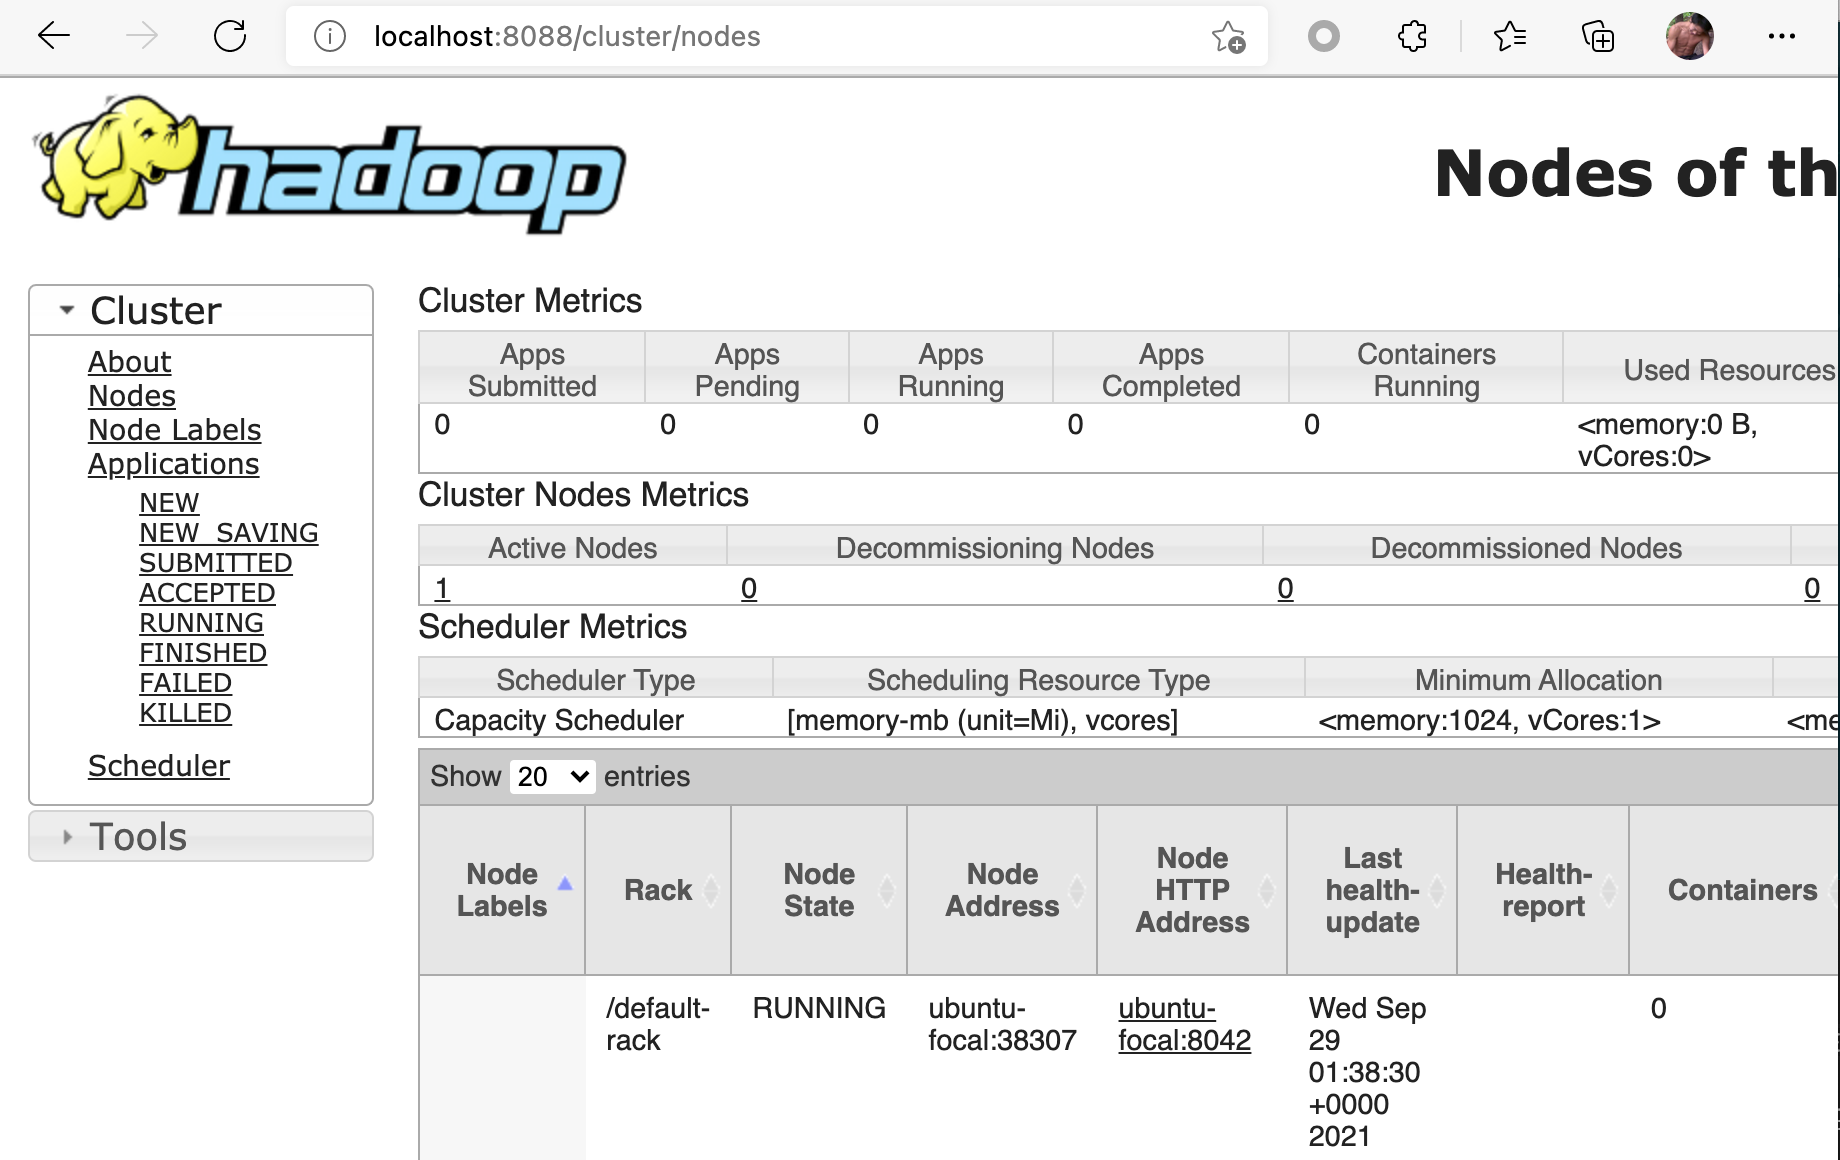
\includegraphics[keepaspectratio,alt={ResourceManager}]{images/Hadoop-8088.png}}
\caption{ResourceManager}
\end{figure}

\begin{figure}
\centering
\pandocbounded{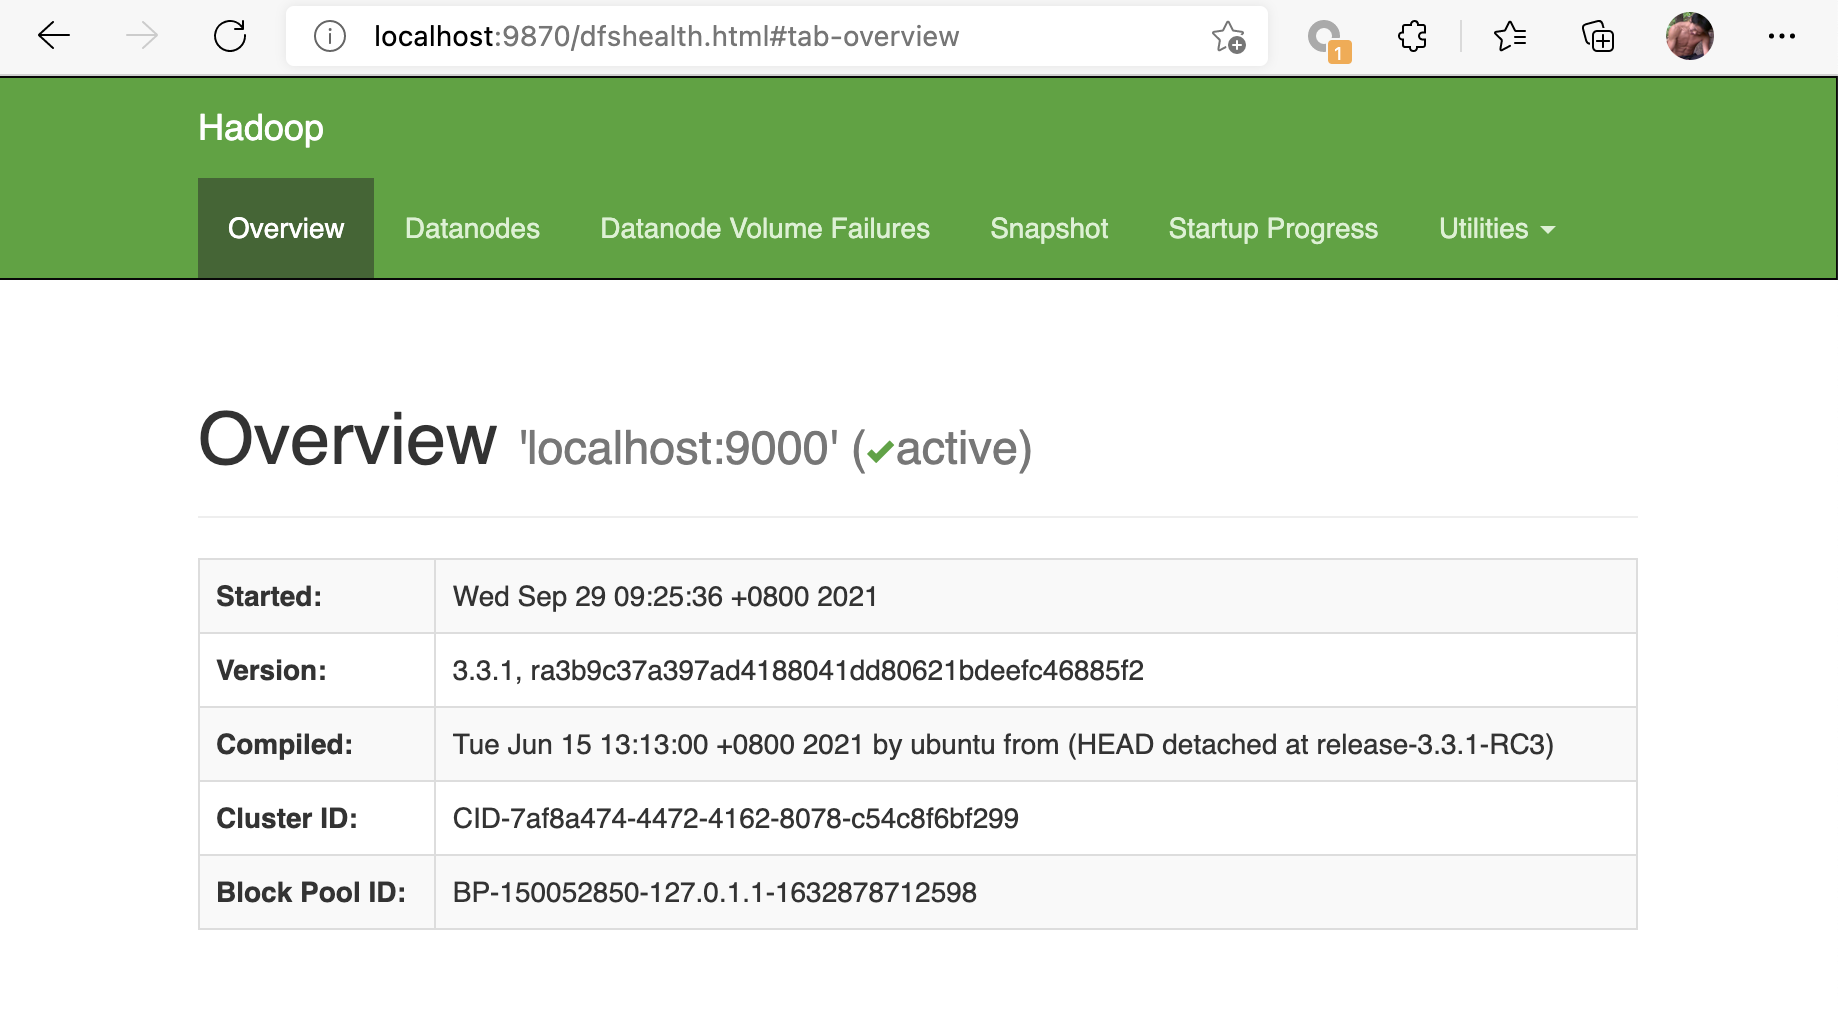
\includegraphics[keepaspectratio,alt={NameNode}]{images/Hadoop-9870.png}}
\caption{NameNode}
\end{figure}

这样就算安装完成了。


\end{document}
